\graphicspath{{./figures}}

\section{PocketQube Unit PCB}

It was decided to order the PQ unit PCB in bulk from an external supplier, due to the higher complexity of the board. In order to begin initial development and testing, a breadboard prototype was initially created using an Arduino Nano. Since the Nano has the same MCU as the designed PCB, the developed software could then simply be flashed onto the PQ unit using an off-board programmer.

The final module is shown in Figures and . On the PCB itself, it was noted that the two required loading capacitors were mistakingly left out for the MCU's crystal oscillator. The MCU's internal 8 MHz clock was therefore used. The board was first bootloaded with an Arduino Nano, and then the programmer circuit in the Figure was developed to flash the board via UART. The programmer consists of a CH340 USB-to-serial module, a reset RC filter, as well as a 3.3V to 5V level converter (since the PocketQube PCB is designed to run at 3.3V).

\begin{figure}[!htb]
  \begin{minipage}{.49\textwidth}
    \centering
    \includegraphics[width=0.85\linewidth]{pqUnitPCB}
    \caption{PQ Unit (front) [right] and programmer [left]}
    \label{fig:pqUnitPCB}
  \end{minipage}
  \begin{minipage}{.49\textwidth}
    \centering
    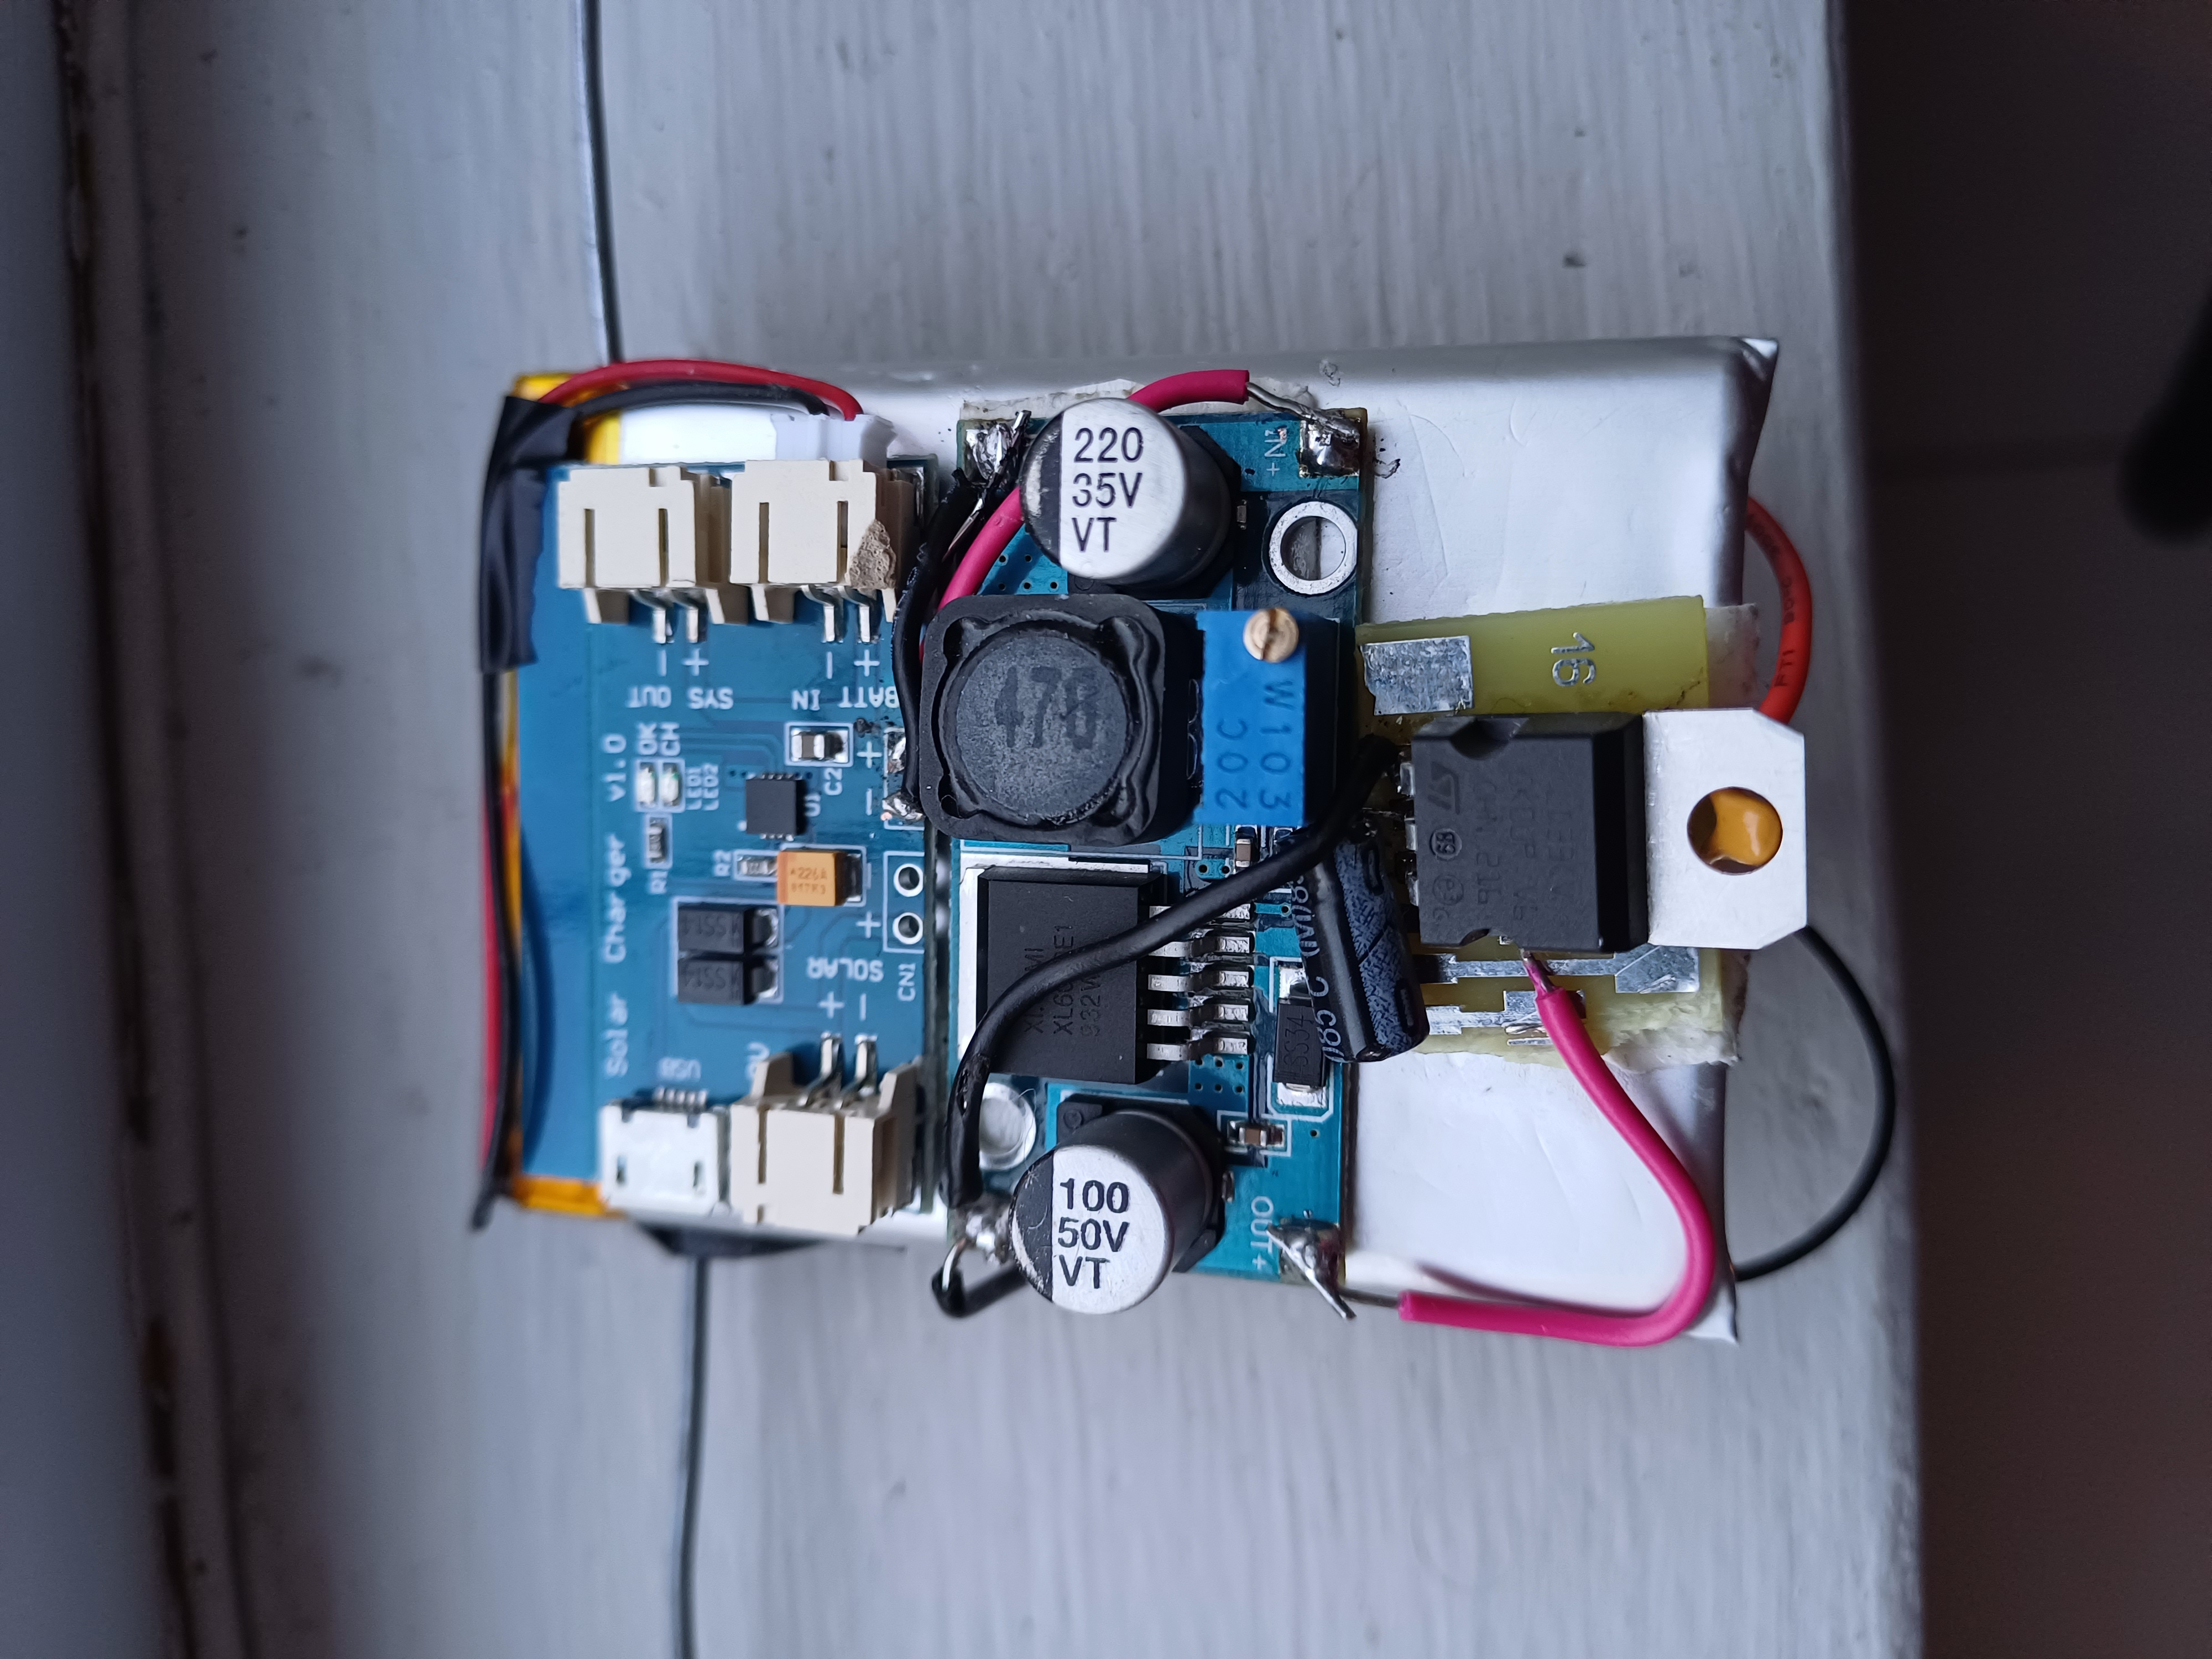
\includegraphics[width=0.85\linewidth]{pqUnitPower}
    \caption{PQ Unit (back)}
    \label{fig:pqUnitPower}
  \end{minipage}
\end{figure}

The board and dipole antenna was mounted onto a LiPo battery. The power section consists of a LiPo charger, a boost converter module, and a 3.3V linear voltage regulator circuit. This section was implemented in order to supply the PocketQube with power through the bus to allowing for testing without being connected to USB power.